% DPF 09 talk on strangeness in nucleon

\documentclass[10pt]{beamer}
\usepackage{amsmath}
\usepackage{mathtools}
%\documentclass[12pt]{beamerthemeSam.sty}
\usepackage{epsf}
%\usepackage{pstricks}
%\usepackage[orientation=portrait,size=A4]{beamerposter}
\geometry{paperwidth=160mm,paperheight=120mm}
%DT favorite definitions
\def\LL{\left\langle}	% left angle bracket
\def\RR{\right\rangle}	% right angle bracket
\def\LP{\left(}		% left parenthesis
\def\RP{\right)}	% right parenthesis
\def\LB{\left\{}	% left curly bracket
\def\RB{\right\}}	% right curly bracket
\def\PAR#1#2{ {{\partial #1}\over{\partial #2}} }
\def\PARTWO#1#2{ {{\partial^2 #1}\over{\partial #2}^2} }
\def\PARTWOMIX#1#2#3{ {{\partial^2 #1}\over{\partial #2 \partial #3}} }

\def\rightpartial{{\overrightarrow\partial}}
\def\leftpartial{{\overleftarrow\partial}}
\def\diffpartial{\buildrel\leftrightarrow\over\partial}

\def\BI{\begin{itemize}}
\def\EI{\end{itemize}}
\def\BE{\begin{displaymath}}
\def\EE{\end{displaymath}}
\def\BEA{\begin{eqnarray*}}
\def\EEA{\end{eqnarray*}}
\def\BNEA{\begin{eqnarray}}
\def\ENEA{\end{eqnarray}}
\def\EL{\nonumber\\}


\newcommand{\map}[1]{\frame{\frametitle{\textbf{Course map}}
\centerline{\includegraphics[height=0.86\paperheight]{../../map/#1.png}}}}
\newcommand{\wmap}[1]{\frame{\frametitle{\textbf{Course map}}
\centerline{\includegraphics[width=0.96\paperwidth]{../../map/#1.png}}}}

\newcommand{\etal}{{\it et al.}}
\newcommand{\gbeta}{6/g^2}
\newcommand{\la}[1]{\label{#1}}
\newcommand{\ie}{{\em i.e.\ }}
\newcommand{\eg}{{\em e.\,g.\ }}
\newcommand{\cf}{cf.\ }
\newcommand{\etc}{etc.\ }
\newcommand{\atantwo}{{\rm atan2}}
\newcommand{\Tr}{{\rm Tr}}
\newcommand{\dt}{\Delta t}
\newcommand{\op}{{\cal O}}
\newcommand{\msbar}{{\overline{\rm MS}}}
\def\chpt{\raise0.4ex\hbox{$\chi$}PT}
\def\schpt{S\raise0.4ex\hbox{$\chi$}PT}
\def\MeV{{\rm Me\!V}}
\def\GeV{{\rm Ge\!V}}

%AB: my color definitions
%\definecolor{mygarnet}{rgb}{0.445,0.184,0.215}
%\definecolor{mygold}{rgb}{0.848,0.848,0.098}
%\definecolor{myg2g}{rgb}{0.647,0.316,0.157}
\definecolor{abtitlecolor}{rgb}{0.0,0.255,0.494}
\definecolor{absecondarycolor}{rgb}{0.0,0.416,0.804}
\definecolor{abprimarycolor}{rgb}{1.0,0.686,0.0}
\definecolor{Red}           {cmyk}{0,1,1,0}
\definecolor{Grey}           {cmyk}{.7,.7,.7,0}
\definecolor{Lg}           {cmyk}{.4,.4,.4,0}
\definecolor{Blue}          {cmyk}{1,1,0,0}
\definecolor{Green}         {cmyk}{1,0,1,0}
\definecolor{Brown}         {cmyk}{0,0.81,1,0.60}
\definecolor{Black}         {cmyk}{0,0,0,1}

\usetheme{Madrid}


%AB: redefinition of beamer colors
%\setbeamercolor{palette tertiary}{fg=white,bg=mygarnet}
%\setbeamercolor{palette secondary}{fg=white,bg=myg2g}
%\setbeamercolor{palette primary}{fg=black,bg=mygold}
\setbeamercolor{title}{fg=abtitlecolor}
\setbeamercolor{frametitle}{fg=abtitlecolor}
\setbeamercolor{palette tertiary}{fg=white,bg=abtitlecolor}
\setbeamercolor{palette secondary}{fg=white,bg=absecondarycolor}
\setbeamercolor{palette primary}{fg=black,bg=abprimarycolor}
\setbeamercolor{structure}{fg=abtitlecolor}

\setbeamerfont{section in toc}{series=\bfseries}

%AB: remove navigation icons
\beamertemplatenavigationsymbolsempty
\title{
  \textbf {Elastic collisions and practice problems}\\
%\centerline{}
%\centering
%\vspace{-0.0in}
%\includegraphics[width=0.3\textwidth]{propvalues_0093.pdf}
%\vspace{-0.3in}\\
%\label{intrograph}
}

\author[W. Freeman] {Physics 211\\Syracuse University, Physics 211 Spring 2015\\Walter Freeman}

\date{\today}

\begin{document}

\frame{\titlepage}

\frame{\frametitle{\textbf{Announcements}}
\BI
\item{If your exam was misgraded, grade appeals will be handled the same way as before (and faster!); turn them in to me by tomorrow}
\item{Extended Friday office hours for homework help: 10-12, then 1-3 (remember, it's due Wednesday)}
\item{Today:}
  \BI
\item{A bit more on the types of collisions}
\item{A bit of ugly math (bear with me; worst math of the semester!)}
\item{Lots of practice problems}
  \EI
\EI
}

\frame{\frametitle{\textbf{Ask a Physicist: the LHC}}
  \centerline{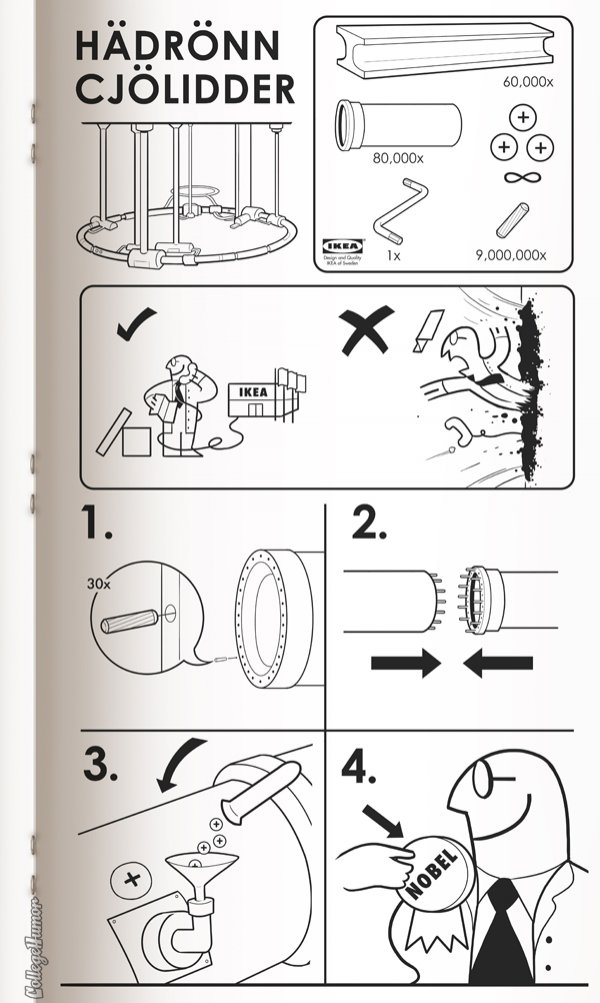
\includegraphics[width=0.3\textwidth]{ikea-lhc.jpg}}
}

\frame{\frametitle{\textbf{Collisions, in more detail}}
  \BI
\item{Last time, we saw that conservation of momentum helps us understand {\bf collisions} and {\bf explosions}}
\item{If we know nothing else, we often don't have enough equations to solve for our unknowns...}
\item{One dimension: one equation, often two unknowns}
    \BI
  \item{$m_1 v_{1,i} + m_2 v_{2,i} = m_1 v_{1,f} + m_2 v_{2,f}$}
      \EI
      \item{Two dimensions: two equations, often four unknowns}
        \BI
      \item{$m_1 v_{1,x,i} + m_2 v_{2,x,i} = m_1 v_{1,x,f} + m_2 v_{2,x,f}$}
      \item{$m_1 v_{1,y,i} + m_2 v_{2,y,i} = m_1 v_{1,y,f} + m_2 v_{2,y,f}$}
        \EI
      \item{Last time we studied {\bf inelastic collisions}, which reduces the number of unknowns: the objects stick together}
      \item{What else might happen?}
          \EI
        }


\frame{\frametitle{\textbf{Three types of collisions, informally}}
  \Large
  \BI
\item{Completely inelastic collisions: ``things stick together''}
\item{Partially inelastic collisions: ``things bounce a bit''}
\item{Completely elastic collisions: ``maximum amount of bounce''}
  \EI
}

\frame{\frametitle{\textbf{Three types of collisions, formally}}
  \large
  \BI
\item{Completely inelastic collisions: things stick together; maximum amount of KE lost}
\item{Partially inelastic collisions: things bounce a bit; lesser amount of KE lost}
\item{Completely elastic collisions: maximum bounce; {\bf no KE lost}}
  \EI
}

\frame{\frametitle{\textbf{Understanding elastic collisions, in one dimension}}
  \large
  A particular situation comes up often: an object with mass $m_1$ and velocity $v_{1i}$ collides elastically with an object with mass $m_2$ at rest.

  \bigskip
  
  What are their final velocities?
  
  \bigskip

\pause\bigskip

  We know both {\bf momentum} and {\bf kinetic energy} are conserved.

\bigskip

  \begin{align*}
    m_1 v_{1i} + m_2 (0) &= m_1 v_{1f} + m_2 v_{2f} \\
    \frac{1}{2} m_1 v_{1i}^2 &= \frac{1}{2} m_1 v_{1f}^2 + \frac{1}{2} m_2 v_{2f}^2
  \end{align*}

\bigskip

  In principle, we have two equations and two unknowns, and can just solve this. But the math is a bit hairy. Bear with me for just a bit (on document camera)
}

\frame{\frametitle{\textbf{Understanding elastic collisions, in one dimension}}
  
    \begin{align*}
          m_1 v_{1i} + m_2 (0) &= m_1 v_{1f} + m_2 v_{2f} \\
      \\
          \frac{1}{2} m_1 v_{1i}^2 &= \frac{1}{2} m_1 v_{1f}^2 + \frac{1}{2} m_2 v_{2f}^2 
        \end{align*}

\bigskip
\bigskip

        Coming out the other end, you get:

\bigskip
\bigskip

\Large
        \begin{align*}
          v_{1f} &= \frac{m_1 - m_2}{m_1 + m_2} v_{1i} \\
          \\
          v_{2f} &= \frac{2m_1}{m_1 + m_2} v_{1i} 
        \end{align*}
      }

      \frame{\frametitle{\textbf{What should you know about this?}}
        \BI
      \item{This is a canned solution to a particular problem}
      \item{Usually I discourage just remembering things like this...}
      \item{... but this one is often useful, and the derivation isn't illuminating}
        \EI
        \begin{align*}
          v_{1f} &= \frac{m_1 - m_2}{m_1 + m_2} v_{1i} \\
          \\
          v_{2f} &= \frac{2m_1}{m_1 + m_2} v_{1i} 
        \end{align*}

        \BI
      \item{If $m_1 >> m_2$, then we basically have:}
        \begin{align*}
          v_{1f} &\approx v_{1i} \\
          \\
          v_{2f} &\approx 2v_{1i} 
        \end{align*}
      \item{If $m_1 << m_2$, then we basically have:}
        \begin{align*}
          v_{1f} &\approx -v_{1i} \\
          \\
          v_{2f} &\approx 2 \frac{m_1}{m_2}v_{1i} 
        \end{align*}
      \item{Looking at limiting cases like this is a huge part of physics!}
        \EI
      }

      \frame{\frametitle{\textbf{What should you know about this?}}
\large
        \BI
      \item{You will {\it not} need to memorize these; they're on page 266 of your book, or here}
      \item{You do need to know where they come from: {\bf conservation of momentum + conservation of KE}}
        \EI
      }




\frame{\frametitle{\textbf{Sample problems: a 1D collision (for 9:30)}}
  \Large
  A train car with a mass $m$ is at rest on a track. Another train car also of mass $m$ is moving toward it with a velocity $v_0$ when it is a distance $d$ away. 
  The first car hits the second and couples to it; the cars roll together until friction brings them to a stop.

\bigskip


If the coefficient of rolling friction is $\mu_r$, how far do they roll after the collision?

\pause

\bigskip
\bigskip
\bigskip


Method: use conservation of momentum to understand the collision; use other methods to understand before and after!

}

\frame{\frametitle{\textbf{Sample problems}}
  \Large
  Three identical train cars, coupled together, are rolling east at speed $v_0$. A fourth car traveling east at $2v_0$ catches up with the
  three and couples to make a four-car train. A moment later, the
  train cars hit a fifth car that was at rest on the tracks, and it couples
  to make a five-car train. What is the speed of the five-car train?

\bigskip

(from textbook; ignore friction)

\bigskip
\bigskip
\bigskip

\pause

Do we care about the order these things happen in?

}

\frame{\frametitle{\textbf{Sample problems}}
  \centerline{ 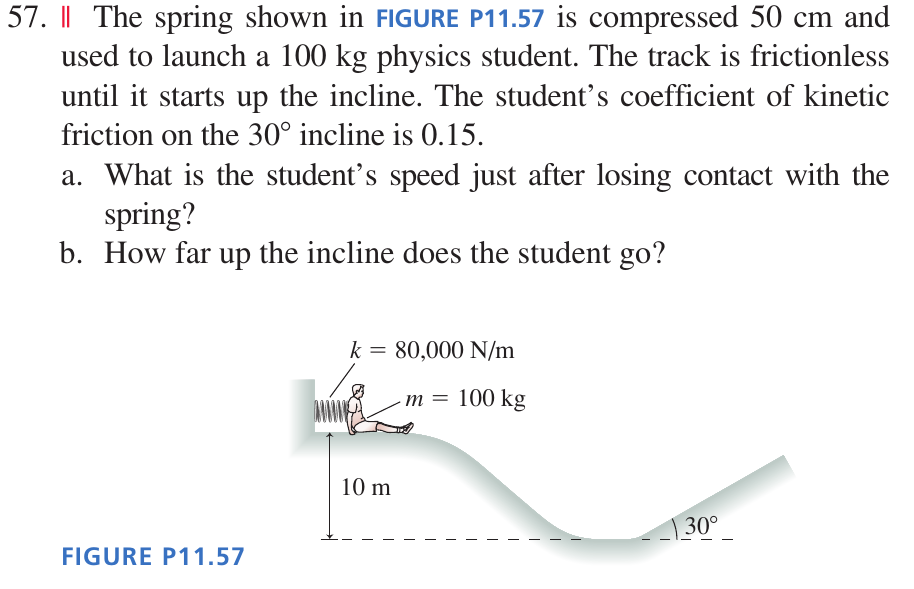
\includegraphics[width=0.6\textwidth]{student-on-spring.png}}
}

\frame{\frametitle{\textbf{Sample problems}}
  
    \Large
  A firecracker in a coconut blows the coconut into three pieces.
 Two pieces of equal mass fly off south and west, perpendicular
 to each other, at speed v0. The third piece has twice the mass
 as the other two. What are the speed and direction of the third
 piece? 
 }



\frame{\frametitle{\textbf{Sample problems}}
  \centerline{ 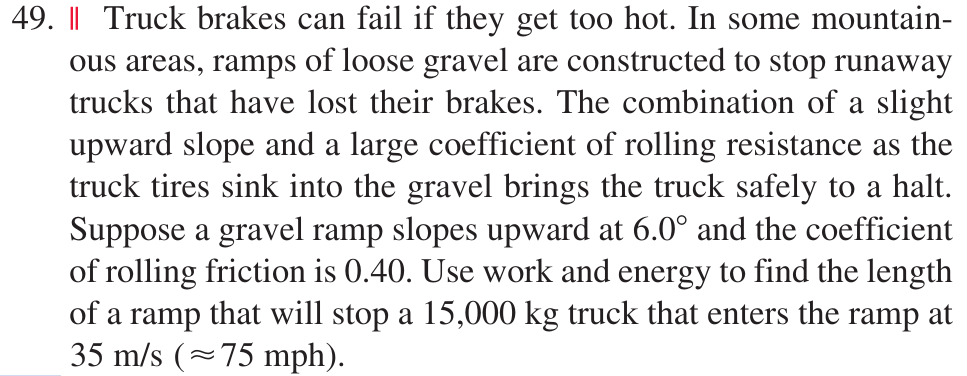
\includegraphics[width=0.6\textwidth]{runaway.png}}
}

\frame{\frametitle{\textbf{Sample problems}}
  \centerline{ 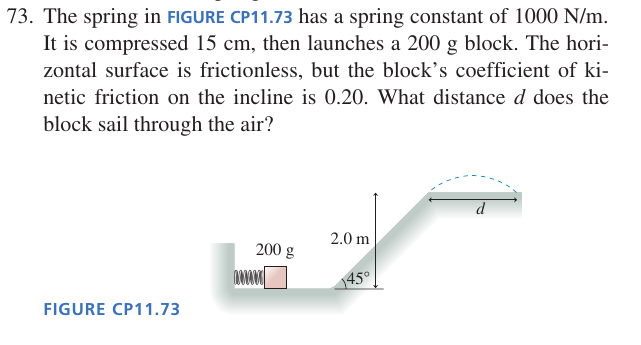
\includegraphics[width=0.6\textwidth]{challenge.png}}
}

\end{document}
